\documentclass[a4paper, 12pt]{book}
\includeonly{chapter01, chapter02, chapter03, chapter04}
\usepackage[a4paper, BCOR1cm]{typearea}
\usepackage[spanish, es-ucroman]{babel}
\usepackage[format=hang, font=small, labelfont=bf, labelsep=endash, width=.9\textwidth]{caption}
\usepackage[color]{changebar}
\usepackage[latin1]{inputenc}
\usepackage[hang, sf]{subfigure}
\usepackage[full]{textcomp}
\usepackage[bf, sf]{titlesec}
\usepackage[nottoc]{tocbibind}
\usepackage[spanish]{varioref}
\usepackage{graphicx}
\usepackage{amsfonts, amsmath, amssymb, calc, color, fancyhdr, hyperref, ifthen, listings, nextpage, textcase}
\usepackage{array, booktabs, tabularx, tabulary, dcolumn, multirow, rotating, threeparttable}
\titleformat{\part}[display]{\centering\huge\sffamily\bfseries}{\partname\ \thepart}{.5\baselineskip}{}
\hypersetup{%
	pdftitle=Proceso de adquisici�n y tratamiento de se�ales de %
	ultrasonidos, pdfauthor=Jos� Ram�n Gisbert Valls, pdfcreator=Vim 7.2,%
	pdfstartview=FitH, colorlinks=true, pdfdisplaydoctitle=true,%
	naturalnames=true, breaklinks=true, bookmarksopen=true,%
	linkcolor=black%
}
\fancyhf{}
\fancyhead[RO, LE]{\sffamily\bfseries\thepage}
\fancyhead[LO]{\sffamily\nouppercase{\rightmark}}
\fancyhead[RE]{\sffamily\nouppercase{\leftmark}}
\pagestyle{fancy}
\fancypagestyle{plain}{%
	\fancyhf{}
	\renewcommand\headrulewidth{0pt}
}
\lstloadlanguages{Matlab}
\lstset{language=Matlab, extendedchars=true, breaklines}
\cbcolor{red}
\labelformat{equation}{ecuaci�n~#1}
\labelformat{figure}{figura~#1}
\labelformat{section}{secci�n~#1}
\labelformat{subsection}{secci�n~#1}
\labelformat{subsubsection}{secci�n~#1}
\labelformat{table}{cuadro~#1}
\labelformat{footnote}{#1\protect\iscurrentchapter{\thechapter}}
\setkeys{Gin}{width=.8\linewidth}
\graphicspath{{./pictures/}{../pictures/}}
\DeclareGraphicsRule{.1}{mps}{*}{}
\DeclareCaptionLabelFormat{cont}{#1~#2\alph{ContinuedFloat}}
\captionsetup[ContinuedFloat]{labelformat=cont}
\newcommand\iscurrentchapter[1]{\ifthenelse{\equal{#1}{\thechapter}}{  en el Cap�tulo~#1}}
\newcommand\matlab{\textsc{matlab}}
\newcommand\kpci{\textsc{kpci}-3108}
\newcommand\datx{\emph{Data Acquisition Toolbox}}
\newcommand\minifootnoterule{\vspace*{-3pt}\hrule width 2in height 0.4pt \vspace*{2.2pt}}
\newcommand\minifootnotemark[1]{\makebox[1.8em][l]{\mbox{\textsuperscript{\normalfont#1}}}}
\newcommand\minifootnotetext[2]{\makebox[1.8em][r]{\mbox{\textsuperscript{\normalfont#1}}}\footnotesize#2\par\noindent}
\newcommand\miniit[1]{\begin{itemize} #1 \end{itemize}}
\renewcommand\chaptermark[1]{\markboth{#1}{}}
\renewcommand\cleardoublepage{\cleartooddpage[\thispagestyle{empty}]}
\renewcommand\tnote[1]{\makebox[1.8em][l]{\mbox{\textsuperscript{\normalfont#1}}}}
\renewcommand\TPTnoteLabel[1]{\makebox[1.8em][r]{\mbox{\textsuperscript{\normalfont#1}}}}
\newcolumntype{d}[1]{D{,}{,}{#1}}
\newcolumntype{+}{D{/}{\mbox{\ --\ }}{5}}
\begin{document}

\frontmatter

\tableofcontents

\listoftables

\listoffigures

\include{chapter01}


\mainmatter

\part{Sistema de adquisici�n y procesado de se�ales}

\chapter{Tarjeta de adquisici�n de se�ales}

Para preparar el sistema de adquisici�n y procesado de se�ales se dispuso en origen de una tarjeta de adquisici�n con interfaz \textsc{pci}. En concreto se ha empleado el modelo \kpci{} de la casa \emph{Keithley}. A continuaci�n se exponen las caracter�sticas t�cnicas que ofrece este dispositivo, en apartados siguientes una breve descripci�n funcional y la disposici�n y uso de los puertos presentes en el mencionado dispositivo.


\section{Caracter�sticas t�cnicas del hardware}

La tarjeta \kpci{} puede emplearse para la adquisici�n y conversi�n de se�ales anal�gicas en se�ales digitales, para sintetizar se�ales anal�gicas a partir de se�ales digitales previamente generadas o almacenadas, o ---gracias a sus 32 puertos digitales de prop�sito general--- trabajar con se�ales digitales.\par
El primer bloque del sistema electr�nico de medida propuesto, es decir el sistema de adquisici�n y procesado de se�ales, tan s�lo requiere de la funci�n de adquisici�n anal�gica de la tarjeta. Por ello, de entre todas las caracter�sticas del dispositivo, se ha cre�do conveniente resumir a continuaci�n aquellas que tienen relaci�n directa con dicha funci�n. Para obtener informaci�n detallada sobre la relaci�n que estos atributos guardan con el proceso de adquisici�n de se�ales anal�gicas en la tarjeta \kpci{}, rec�rrase a la \vref{sec:functional-description}.

\begin{itemize}
	\item El m�dulo de adquisici�n anal�gica dispone de 16 puertos f�sicos.
	\item La impedancia de entrada equivalente de cada puerto es aproximadamente igual a una capacidad de 200 pF en serie con una resistencia de valor inferior, pero aproximadamente igual, a 1 K$\Omega$.
	\item En condiciones �ptimas, es posible conseguir un rendimiento m�ximo de 100 KS/s (cien mil operaciones de conversi�n por segundo). Este valor est� sujeto a un error relativo del $0.02 \%$.
	\item La resoluci�n del conversor anal�gico digital es de 16 bits por muestra. El rango de amplitudes en el que opera depende de como est� configurado el modo de adquisici�n.% Este puede ser de 0 a 10 si el modo de adquisici�n es unipolar, o de -10 a 10 si es bipolar.
	\item La cola de muestreo tiene capacidad para hasta 256 canales distintos. Cada uno de los cuales puede configurarse independientemente en t�rminos de ganancia, frecuencia de muestreo, modo de adquisici�n o modo de terminaci�n.
	\item La ganancia, responsable en parte de la resoluci�n con la que se cuantifica las muestras, puede tomar cada ciclo de reloj uno de entre 16 valores posibles. V�ase el cuadro \vref{tab:acquisition-modes}.
	% \item Soporte, tanto en el modo de adquisici�n y conversi�n como en el modo de s�ntesis, para disparo digital externo o controlado por software.
	% \item Selecci�n por software del flanco activo de disparo.
	% \item Capacidad de interrumpir el muestreo tras un determinado n�mero de ciclos despu�s del disparo. La cantidad de ciclos puede controlarse por software.
\end{itemize}


\section{Descripci�n funcional}\label{sec:functional-description}

Es necesario programar el comportamiento de la tarjeta de adquisici�n antes de ponerla en funcionamiento. Desde la cola de muestreo se controlan los principales aspectos del proceso de adquisici�n, como por ejemplo, en que instantes se encuentra activo.\par% La configuraci�n correspondiente al proceso de adquisici�n anal�gica reside en su pr�ctica totalidad en la cola de muestreo. Desde la cola se controlan los principales aspectos de este proceso, como por ejemplo, en que instantes se encuentra activo.\par
La cola de muestreo, como su propio nombre indica, es una estructura de datos ordenada. Se encuentra almacenada en una memoria \textsc{ram} de 256 entradas que forma parte del hardware de la tarjeta. En el \vref{tab:sample-queue} puede verse una representaci�n de un ejemplo de la cola de muestreo.\par

\begin{table}[h]
	\begin{center}
	\begin{threeparttable}
	\begin{tabular}{lccccccccc}
		\toprule
		Posici�n en la cola & 1 & 2 & 3 & 4 %
		& \multicolumn{2}{c}{$\cdots$} & 254 & 255 & 256 \\
		\midrule
		N�mero de canal & 15 & 15 & 02 & 02 %
		& \multicolumn{2}{c}{$\cdots$} & 17 & 13 & 01 \\
		N�mero de puerto\minifootnotemark{a, b} & 07 & 07 & 11 & 11 %
		& \multicolumn{2}{c}{$\cdots$} & 07 & 09 & 01 \\
		Ganancia & 1 & 1 & 40 & 40 %
		& \multicolumn{2}{c}{$\cdots$} & 200 & 8 & 80 \\
		Modo de adquisici�n\minifootnotemark{c} & $\pm$ & $\pm$ & $+$ & $+$ %
		& \multicolumn{2}{c}{$\cdots$} & $\pm$ & $+$ & $\pm$ \\
		Modo de terminaci�n\minifootnotemark{d} & \textsc{d} & \textsc{d} & \textsc{ts} %
		& \textsc{ts} & \multicolumn{2}{c}{$\cdots$} & \textsc{d} & \textsc{ts} %
		& \textsc{ts} \\
		\bottomrule
	\end{tabular}
	\vspace{\skip\footins}
	\minifootnoterule
		\minifootnotetext{a}{Si el canal es diferencial el n�mero de puerto identifica un par de puertos. Un canal diferencial no puede estar asociado a un n�mero de puerto superior a 07.}
		\minifootnotetext{b}{Dos canales pueden estar relacionados con los mismos puertos f�sicos.}
		\minifootnotetext{c}{$\pm$ configuraci�n bipolar; $+$ configuraci�n unipolar}
		\minifootnotetext{d}{\textsc{d} canal diferencial; \textsc{ts} canal monoterminal}
	\end{threeparttable}
	\end{center}
	\caption{Ejemplo de cola de muestreo}
	\label{tab:sample-queue}
\end{table}

Cada entrada en la memoria \textsc{ram} se identifica con una posici�n en la cola. Las posiciones en la cola pueden encontrarse vac�as o estar ocupadas por un canal. Varias posiciones en la cola, consecutivas o no, pueden estar ocupadas por un mismo canal. Por tanto, la cola puede estar ocupada, como m�ximo, por 256 canales independientes.\par
Las posiciones ocupadas contienen informaci�n correspondiente al canal y a los atributos asociados a este. Un canal es una entidad l�gica que relaciona un puerto f�sico con un b�ffer de informaci�n y una serie de atributos. Durante el proceso de adquisici�n un puntero recorre las distintas posiciones de la cola, una a una y en orden. El canal activo, aquel que ocupa la posici�n a la que apunta el puntero en cada ciclo de reloj, determina tres cosas:

\begin{itemize}
	% \footnote{Por convenio se ha elegido hablar de una sola se�al que entra al amplificador. Si se ha hecho esta elecci�n, es porque si bien al amplificador pueden entrar una o dos se�ales simult�neamente desde sendos puertos, tal y como se ver� m�s adelante, esto no supone otra diferencia para el proceso que la expuesta en la secci�n \vref{sec:termination-modes}
	\item De qu� puerto debe proceder la se�al anal�gica\footnote{Por convenio se ha elegido hablar de una sola se�al que entra al amplificador. Si se ha hecho esta elecci�n, es porque si bien al amplificador pueden entrar una o dos se�ales simult�neamente, esto no supone otra diferencia para el proceso que la expuesta en la secci�n \vref{sec:termination-modes}. Es por ello, y para mantener la claridad, que se ha omitido esta posibilidad.} que llega al amplificador de instrumentaci�n interno de la tarjeta.
	\item D�nde, en qu� b�ffer, debe almacenarse el valor resultante de muestrear y cuantificar esta se�al.% las muestras cuantificadas resultantes del proceso.
	\item Por �ltimo, los atributos asociados al canal: ganancia, modo de adquisici�n y modo de terminaci�n; indican, respectivamente, cu�l debe ser la ganancia del amplificador de instrumentaci�n, cu�l debe ser el rango de trabajo del conversor anal�gico digital, y qu� se debe conectar a los terminales de entrada del amplificador de instrumentaci�n. Se da m�s informaci�n al respecto en apartados subsiguientes.% la polaridad de las muestras y el n�mero de terminales de entrada, uno o dos dependiendo de si la adquisici�n es diferencial o no, durante el ciclo actual.
\end{itemize}

Para concluir el apartado cabe remarcar lo siguiente. Es posible inferir dos cosas de esta mec�nica de funcionamiento basada en la cola. Una de ellas es que el proceso de adquisici�n afecta a una sola se�al cada vez. Y la segunda, que la frecuencia de muestreo ligada a un canal depende de dos factores, de la velocidad de la se�al de reloj, y de la cantidad de veces que un canal aparece repetido en la cola.


\subsection{M�todos de entrada}

La \kpci{} permite dos modos de adquisici�n y dos modos de terminaci�n. Aprender a diferenciar cuando es oportuno seleccionar entre cada uno de ellos beneficiar� la calidad de la se�al digital resultante.


\subsubsection{Modos de adquisici�n}
Una se�al es bipolar cuando toma valores positivos y negativos. Por el contrario, se distingue a las se�ales unipolares porque todos sus valores mantienen la misma polaridad, ya sea �sta positiva o negativa. Para cada canal, debe configurarse el modo de adquisici�n como bipolar o unipolar\footnote{La tarjeta \kpci{} s�lo admite se�ales unipolares de polaridad positiva.} atendiendo a la se�al de inter�s.\par
% El modo de adquisici�n unipolar presenta la ventaja de que en dicho modo pr�cticamente se duplica la resoluci�n de las muestras. Manteniendo la ganancia, se reduce el rango de trabajo a la mitad. El paso correspondiente a una cuantificaci�n de 16 bits se reduce de igual manera y, por tanto, aumenta la precisi�n.
Si se sabe a ciencia cierta que la se�al de entrada es unipolar debe emplearse el modo de adquisici�n unipolar. De ese modo, se duplica la resoluci�n del conversor anal�gico digital.

\begin{table}[hbt]
	\begin{center}
		\begin{tabular}{>{\raggedleft}p{1.2cm}d{5.2}d{3.1}+d{3.1}}
			\toprule
			& \multicolumn{2}{c}{Bipolar} & \multicolumn{2}{c}{Unipolar} \\
			\cmidrule(r){2-3}\cmidrule(l){4-5}
			\multicolumn{1}{c}{Ganancia}
			& \multicolumn{1}{c}{Rango ($\pm\text{V}$)} %
			& \multicolumn{1}{c}{Precisi�n ($\mu\text{V}$)} %
			& \multicolumn{1}{c}{Rango (V)} %
			& \multicolumn{1}{c}{Precisi�n ($\mu\text{V}$)} \\
			\midrule
			1 & 10,0 & 305 & 0/$10,0$ & 153 \\
			2 & 5,0 & 153 & 0/$5,0$ & 76 \\
			4 & 2,5 & 76 & 0/$2,5$ & 38 \\
			8 & 1,25 & 38 & 0/$1,25$ & 19 \\
			10 & 1,0 & 31 & 0/$1,0$ & 15 \\
			\\
			& \multicolumn{2}{c}{Bipolar} & \multicolumn{2}{c}{Unipolar} \\
			\cmidrule(r){2-3}\cmidrule(l){4-5}
			\multicolumn{1}{c}{Ganancia}
			& \multicolumn{1}{c}{Rango ($\pm\text{mV}$)} %
			& \multicolumn{1}{c}{Precisi�n ($\mu\text{V}$)} %
			& \multicolumn{1}{c}{Rango (mV)} %
			& \multicolumn{1}{c}{Precisi�n ($\mu\text{V}$)} \\
			\midrule
			20 & 500 & 15 & 0/500 & 7,6 \\
			40 & 250 & 7,6 & 0/250 & 3,8 \\
			80 & 125 & 3,8 & 0/125 & 1,9 \\
			100 & 100 & 3,1 & 0/100 & 1,5 \\
			200 & 50 & 1,5 & 0/50 & 0,8 \\
			400 & 25 & 0,8 & 0/25 & 0,4 \\
			800 & 12,5 & 0,4 & 0/$12,5$ & 0,2 \\
			\bottomrule
		\end{tabular}
		\caption{Relaci�n entre ganancia, rango de trabajo y resoluci�n seg�n el modo de adquisici�n}
	\end{center}
	\label{tab:acquisition-modes}
\end{table}


\subsubsection{Modos de terminaci�n}\label{sec:termination-modes}

Internamente, la tarjeta \kpci{} emplea un amplificador de instrumentaci�n diferencial. En principio este hecho implicar�a que a cada canal se asociasen dos puertos f�sicos, uno por cada uno de los dos terminales de entrada del amplificador. No obstante, es posible configurar la tarjeta para que uno de los terminales del amplificador se conecte a masa. En ese caso, el terminal restante se conecta a un puerto f�sico.\par

\begin{figure}[htp]
	\begin{center}
		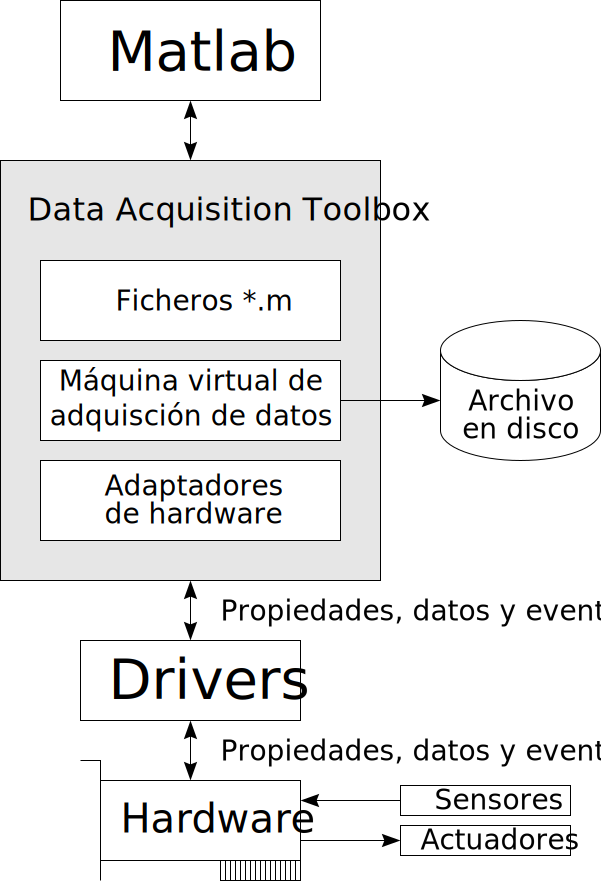
\includegraphics[width=.8\linewidth]{chapter02-01.mps}
	\end{center}
	\caption{Figura que muestra el modo de terminaci�n sencillo. La entrada superior del amplificador de instrumentaci�n se conecta al puerto 9 y la entrada inferior se conecta a masa}
	\label{fig:termination-modes}
\end{figure}

Para hacerlo, cabr�a pensar que es suficiente con modificar el atributo que controla el modo de terminaci�n del canal correspondiente. Al contrario de lo que pudiera parecer, el modo de terminaci�n es una propiedad que no es atribuible al canal, si no que se atribuye a un par de puertos\footnote{Aunque seg�n las especificaciones del fabricante es posible configurar cada par de puertos para que opere seg�n un modo de terminaci�n independiente del resto, \matlab{} s�lo admite un modo de terminaci�n para el conjunto total de puertos.}. En concreto, el modo de terminaci�n afecta a los pares de puertos compuestos por un primero de entre los puertos 0 y 7, y un segundo cuyo n�mero de puerto es igual al del primero m�s 8. De ah� que todos los canales relacionados con el mismo par de puertos deban estar configurados con el mismo modo de terminaci�n, una configuraci�n distinta no est� permitida.\par
Los dos modos de terminaci�n posibles se conocen como: diferencial, si es que la se�al que entra en cada terminal del amplificador procede de cada uno de los puertos del par; sencillo, en caso de que uno de los terminales de entrada del amplificador se conecte a la referencia de tensi�n. En este documento se llama canal diferencial a los canales cuyo modo de terminaci�n sea diferencial, y canal con un s�lo terminal o monoterminal a aquellos para los que el modo de terminaci�n es sencillo. \par
Las ventajas que presenta el uso de uno u otro tipo de canales son comprensibles. Emplear canales con un s�lo terminal permite aplicar el proceso de adquisici�n sobre un mayor n�mero de se�ales simult�neamente. Por el contrario, utilizar canales diferenciales redunda en una mayor inmunidad frente al ruido. Adem�s, los amplificadores diferenciales eliminan de forma inherente la componente en continua.\par
\par


\subsection{Rendimiento}

Se entiende como rendimiento la cantidad m�xima de operaciones de conversi�n que el dispositivo puede realizar por unidad de tiempo. Para que una de estas operaciones contribuya a la medida de rendimiento debe superar un requisito de precisi�n.\par
El rendimiento �ptimo de la tarjeta \kpci{} especificado por el fabricante es de cien mil operaciones por segundo (100 KS/s). No obstante se advierte, para obtener este nivel de rendimiento es necesario alimentar la tarjeta con una fuente de tensi�n ideal. Adem�s, es importante que exista adaptaci�n de impedancias entre el circuito de alimentaci�n y el puerto por el que se quiere introducir la se�al. A�n en estas condiciones el valor proporcionado por la casa Keithley est� sujeto a un error relativo m�ximo del $0.02\%$, el cual supone un error absoluto m�ximo de dos mil operaciones por segundo (2 KS/s).


\subsubsection[Factores limitantes del rendimiento]{Amplificador de instrumentaci�n y p�rdida del rendimiento}

El amplificador de instrumentaci�n interno de la \kpci{} es de ganancia variable. Es posible configurar una ganancia distinta para cada canal. El prop�sito del amplificador es permitir al usuario modificar la amplitud de la se�al que entra al conversor. La intenci�n que se persigue es conseguir que la conversi�n se enfoque en los detalles de la se�al que sean de mayor inter�s y se pierda la m�nima informaci�n posible. Todo ello a�n trabajando simult�neamente con m�ltiples se�ales cuyo rango de amplitudes es con frecuencia muy diferente.\par % El prop�sito de que esto sea as� es conseguir que la amplitud de la se�al que entra al conversor anal�gico digital se encuentre en su rango de trabajo ---de -10 a 10 voltios en configuraci�n bipolar y de 0 a 10 voltios en configuraci�n unipolar--- con independencia de la amplitud de las se�ales que entran a la tarjeta. De esta forma la \kpci{} es capaz de trabajar simult�neamente con varias se�ales de amplitud diferente conservando gran parte de la informaci�n que �stas transportan.
La desventaja que presenta esta configuraci�n ---multiplexor -- amplificador de instrumentaci�n -- conversor--- es una p�rdida de rendimiento que se produce en situaciones determinadas a causa de la intervenci�n del amplificador en la operaci�n de adquisici�n.\par
Cada ciclo de reloj cambia el canal activo y debe cambiar, si es oportuno, la se�al que accede al amplificador. Este proceso no es inmediato. Tras conmutar el multiplexor que precede al amplificador, se da paso al puerto conveniente. No obstante, la se�al que recibe el amplificador presenta, hasta transcurrido un determinado periodo de tiempo, una componente residual de la se�al que se amplific� en el anterior ciclo de reloj. Transcurrido dicho periodo de tiempo la se�al que entra al amplificador se ve libre de esa componente residual y se corresponde �nicamente con la se�al que entrega el multiplexor, se dice que se ha fijado la se�al.\par % La componente residual provoca una p�rdida de precisi�n en los resultados de la conversi�n que en ocasiones pueden perder su validez. Las consecuencias de la aparici�n de componentes residuales
% Y es as� como el amplificador es causa de una p�rdida de rendimiento por medio de las componentes residuales. Si la conversi�n se realiza antes de fijar la se�al, la componente residual no se habr� dispersado completamente y los resultados quedar�n mancillados por su mal
Y es as� como el amplificador es causa de p�rdida de rendimiento, por medio de las componentes residuales. Si la conversi�n se realiza antes de fijar la se�al, el conversor toma un valor de la se�al corrompido por la componente residual de la se�al precedente. Por tanto, la muestra resultante quedar� igualmente corrompida incluso hasta el punto de perder su validez. Las operaciones de conversi�n que tengan como resultado muestras inv�lidas s�lo contribuyen a falsear la medida de rendimiento, haciendo que parezca mayor de lo que en realidad es.\par
El fabricante da a entender que existe una soluci�n de dise�o que resuelve en parte el problema planteado por las componentes residuales. Esta soluci�n consiste en alargar de forma deliberada la duraci�n del ciclo de reloj, de esa forma habr� tiempo suficiente para fijar la se�al. Sin embargo, esta soluci�n presenta dos inconvenientes: no solventa el problema en la totalidad de los casos y es, asimismo, una forma de perder rendimiento. Lo cual conduce inevitablemente a una soluci�n de compromiso, alargar el ciclo de reloj lo suficiente para que en la mayor�a de los casos el efecto de las componentes residuales sobre la precisi�n de la conversi�n no invalide las muestras resultantes y se produzca, por tanto, una ca�da del rendimiento; sin que la duraci�n del nuevo ciclo contribuya por s� misma a una p�rdida notable de rendimiento.\par


\subsubsection{Optimizaci�n del rendimiento}

Como se ha visto, la inclusi�n del amplificador en el dise�o de la tarjeta es causa directa o indirecta de una p�rdida de rendimiento. La magnitud de esa ca�da en el rendimiento depende de la configuraci�n de la cola de muestreo y de la amplitud de la se�al una vez llega �sta al dispositivo de adquisici�n.

\begin{itemize}
	\item Las se�ales cuya tensi�n absoluta se encuentra por debajo de los 100 mV al llegar a la \kpci{} sufren en mayor medida las consecuencias del empleo de un amplificador en la operaci�n de conversi�n. En primer lugar la se�al tarda m�s en fijarse de modo que el rendimiento se reduce a la mitad en las mejores condiciones, de 100 KS/s pasa a 50 KS/s. Esto es debido a que, al ser la amplitud de la se�al y la del ruido comparables, especialmente despu�s de que �ste se vea reforzado por el efecto de las componentes residuales, se genera una mayor incertidumbre.\par
	Por otro lado las se�ales que requieren que el amplificador opere con alta ganancia son las m�s perjudicadas por los problemas que causa el amplificador en configuraciones multiganancia, tal y como se expone a continuaci�n.
	\item Por lo general, el rendimiento se ve afectado de forma m�s pronunciada por el efecto de las componentes residuales en configuraciones multiganancia en las que se encadenan secuencias de canales con ganancia diferente. Una configuraci�n multiganancia de la cola de muestreo implica que en diferentes ciclos de reloj el amplificador act�a con ganancias distintas. Eso con frecuencia significa que el rango en el que se encuentra comprendida la amplitud de las se�ales que est�n entrando al dispositivo de adquisici�n es diferente de una se�al a otra. Cuando as� ocurre puede sucederse en ocasiones que en ciclos de reloj consecutivos entren al amplificador dos se�ales de amplitud diferente, siendo la amplitud de la se�al que ocupa el primer ciclo mucho mayor que la de la otra se�al en el tiempo en el que ambas permanecen a la entrada del dispositivo. Por otro lado, parece l�gico considerar que la componente residual asociada a una se�al cuya amplitud sea predominantemente mayor que la de otra se�al ser� de mayor amplitud inicial y mayor duraci�n temporal que la asociada a la segunda se�al. Por tanto si ocurre como se ha dicho y se tiene en cuenta la base probable que se ha propuesto, cuando la segunda de las se�ales se convierte en la se�al activa la amplitud de la componente residual asociada a la primera de ellas puede ser suficiente, incluso, para enmascararla.\par No s�lo eso, la amplitud de la se�al que llega m�s tarde al amplificador puede ser, en t�rminos absolutos, la mayor parte del tiempo, menor que la de la otra se�al, al ser as� lo m�s probable es que se amplifique empleando un mayor factor de ganancia. De ser as�, la amplitud de la componente residual a la que se enfrenta esta se�al puede provocar en el peor de los casos que el conversor sature y la p�rdida de precisi�n sea mucho mayor. Sea cual sea el caso, es posible observar entonces, que en configuraciones multiganancia las muestras resultantes se obtienen de una conversi�n menos precisa, en especial si se trabaja con se�ales de peque�a amplitud ---tal y como se especific� en el punto anterior--- o si las ganancias configuradas en la cola de muestreo difieren mucho unas de otras. Aplicando la relaci�n entre la validez de las muestras y el rendimiento que se expuso anteriormente, la consecuencia de emplear configuraciones multiganancia es una mayor p�rdida de rendimiento.
	\item En configuraciones monoganancia el uso del amplificador supone una causa indirecta de la ca�da de rendimiento. El dise�o del dispositivo de adquisici�n est� pensado primordialmente para su uso en configuraciones multiganancia, de lo contrario la inclusi�n de un amplificador de ganancia variable en el esquem�tico de la tarjeta ser�a incomprensible. Por la misma raz�n, Keithley adopta una soluci�n de dise�o como la expuesta en el anterior apartado, para tratar de obtener un rendimiento �ptimo en configuraciones multiganancia. Sin embargo, el efecto de las componentes residuales en configuraciones monoganancia es m�nimo y la consecuente p�rdida de rendimiento tambi�n lo es. Por tanto, una soluci�n que consiste en alargar el ciclo de reloj resulta, en configuraciones monoganancia, innecesaria y perjudicial para el rendimiento.
\end{itemize}

Las acciones que el fabricante adopta para tratar de que el usuario obtenga el mayor rendimiento posible del dispositivo no se limitan a aplicar una soluci�n de compromiso en el dise�o de la duraci�n del ciclo de reloj. En el manual de usuario se hacen una serie de recomendaciones orientadas a conseguir este fin.\par % explotar el dispositivo de adquisici�n lo m�ximo posible.\par
Se proponen varias soluciones, la m�s trivial de las cuales pasa por preamplificar todas las se�ales que vayan a ser objeto del proceso de adquisici�n efectuado por la tarjeta consiguiendo que su amplitud var�e en un mismo rango. Si se hace as� ser� suficiente con emplear una configuraci�n monoganancia de la cola de muestreo para minimizar los efectos de las componentes residuales en el rendimiento. Adem�s al preamplificar las se�ales, presentar�n una mejor relaci�n se�al a ruido, es decir, ser�n menos vulnerables al ruido. Aunque buena, esta soluci�n no deja de ser trivial puesto que el amplificador de instrumentaci�n de la tarjeta pierde toda funcionalidad y pasa a ser un estorbo en el proceso de adquisici�n.\par
La soluci�n de car�cter pr�ctico propuesta por Keithley radica en emplear configuraciones <<sensatas>> de la cola de muestreo. Se entiende por configuraci�n sensata aquella que redunda en un rendimiento �ptimo en situaciones normales, situaciones en las que una configuraci�n multiganancia sea imprescindible. Existen dos condiciones que una configuraci�n multiganancia debe cumplir para garantizar un rendimiento �ptimo:

\begin{itemize}
	\item La primera consiste en agrupar canales con distinta ganancia en posiciones consecutivas de la cola, aunque por ello se pierda el orden de muestreo predefinido por el usuario. Si como se presumi� en el apartado anterior, com�nmente dos se�ales que requieren ser amplificadas con el mismo factor de ganancia var�an en el mismo rango de amplitudes, en estas secuencias monoganancia las consecuencias de las componentes residuales en la precisi�n de la conversi�n ser�n m�nimas.
	\item A pesar de emplear una configuraci�n como la anterior todav�a es probable que se produzcan saltos de ganancia, por ejemplo,
\end{itemize}<++>
% Tras adoptar la soluci�n de alargar el ciclo de reloj el fabricante propone soluciones a los problemas planteados por las componentes residuales atendiendo al tipo de situaci�n en el que se producen. Soluci�n trivial, preamplificar las se�ales antes de pasarlas a la tarjeta. Inconveniente, se pierde la funcionalidad del amplificador que s�lo estorba. Soluci�n pr�ctica pasa por emplear una configuraci�n sensata de la cola de muestreo.


\chapter{Aplicaci�n para el control de la tarjeta}



\part{Ensayos no destructivos con ultrasonidos}

\chapter{Fundamentos de los ultrasonidos}

Los ultrasonidos son ondas ac�sticas de naturaleza mec�nica o el�stica como los sonidos. A diferencia de las ondas s�nicas los ultrasonidos se encuentran en una banda de frecuencia superior. Dicha banda parte de los 20 KHz y, carente de un l�mite f�sico, llega hoy hasta los 1000 MHz debido a limitaciones tecnol�gicas. Las frecuencias empleadas en los ensayos no destructivos se encuentran entre los 20 KHz y los 25 MHz. Cabe remarcar que las propiedades de las ondas ac�sticas se mantienen invariantes con la frecuencia, y por tanto, son comunes dentro del espectro ac�stico.\par
Las ondas ultras�nicas son perturbaciones mec�nicas que viajan a trav�s de un medio el�stico, por tanto, la condici�n primordial para que las ondas ultras�nicas se propaguen a trav�s de un medio es que este contenga fracciones de materia tales como �tomos o mol�culas susceptibles de vibrar. El medio determina tambi�n que modos de propagaci�n pueden adoptar las ondas ultras�nicas que se propagan a su trav�s. Frecuentemente se asocia un nombre caracter�stico a las ondas ultras�nicas en funci�n del modo en el que se propagan por el medio. A continuaci�n se exponen los modos de propagaci�n de mayor relevancia.

\begin{itemize}
	\item Las \emph{ondas longitudinales}, tambi�n llamadas \emph{ondas de presi�n o compresi�n}, son aquellas que oscilan en la direcci�n de propagaci�n. Al contrario que el resto de modos de propagaci�n que s�lo se dan en s�lidos, el modo longitudinal puede estar presente tambi�n en l�quidos y gases.
	\item En las \emph{ondas transversales o de cizalladura} las oscilaciones se producen en la direcci�n perpendicular a la direcci�n de propagaci�n.
	\item Las \emph{ondas de superficie} se propagan �nicamente a trav�s de s�lidos semi"=infinitos cuya superficie sea plana o curva y siempre siguiendo las irregularidades del contorno del mismo.
	\item Las \emph{ondas de Lamb o de chapa} son propias de medios s�lidos en los que el espesor es del mismo orden que la longitud de onda, provocan la vibraci�n de todo el material.
\end{itemize}

La energ�a ac�stica que se propaga por un medio se manifiesta en forma de presi�n ac�stica, esta a su vez define el campo ac�stico. La presi�n ac�stica se define como:

\begin{equation}
	p = Z\cdot v
	\label{eq:presion-acustica}
\end{equation}

Ecuaci�n en la que $v$ representa la velocidad de vibraci�n y $Z$ la impedancia ac�stica. La impedancia ac�stica es una medida de con que resistencia se oponen los elementos de masa de un medio a la vibraci�n provocada por las ondas ac�sticas, en ning�n caso da una relaci�n de la resistencia con la que el medio se opone a la propagaci�n de la onda ac�stica. Es una constante del medio que aumenta con la cohesi�n de sus mol�culas, y puede expresarse en funci�n de la densidad $\rho_0$ y de la velocidad de propagaci�n de las ondas ultras�nicas en dicho medio $c$.

\begin{equation}
	Z = \rho_0\cdot c
	\label{eq:impedancia-acustica}
\end{equation}

\section{Campo ac�stico generado por un transductor}

La excitaci�n el�ctrica de un transductor produce una onda de presi�n que se propaga en el medio siguiendo las leyes f�sicas de la propagaci�n de ondas y, en particular, los principios de superposici�n de Huygens\footnote{El tratamiento que se da en esta secci�n a los transductores de ultrasonidos es similar al que la teor�a de antenas da a las antenas de apertura conocidas como bocinas, para un mayor detalle consultar el texto de Stutzman y Thiele}. Se denomina campo ac�stico a la distribuci�n temporal y espacial de la presi�n ac�stica a la que se someten las part�culas materiales del medio en el que se propagan las ondas ac�sticas. Las caracter�sticas del campo ac�stico dependen de aspectos geom�tricos del transductor.


\end{document}
